\documentclass[aspectratio=169]{beamer}
\usepackage[T1]{fontenc}
\usepackage[french]{babel}
\usepackage{booktabs}

\usetheme{Madrid}
\usecolortheme{beaver}
\setbeamertemplate{navigation symbols}{}

\title{{{TITLE}}}
\subtitle{Sous-titre de la présentation}
\author{{{AUTHOR}}}
\institute{Établissement}
\date{\today}

\begin{document}

\begin{frame}
  \titlepage
\end{frame}

\begin{frame}{Plan}
  \tableofcontents
\end{frame}

\section{Introduction}

\begin{frame}{Une diapositive}
  Chaque diapositive est un environnement \texttt{frame}.
  \begin{itemize}
    \item Les listes s'affichent en entier\ldots
    \item<2-> \ldots ou un élément à la fois, avec \texttt{<2->}.
  \end{itemize}
\end{frame}

\section{Contenu}

\begin{frame}{Deux colonnes}
  \begin{columns}
    \column{0.5\textwidth}
    Le texte à gauche, une figure ou un tableau à droite.
    \begin{block}{À retenir}
      Les blocs mettent une idée en valeur.
    \end{block}

    \column{0.45\textwidth}
    \centering
    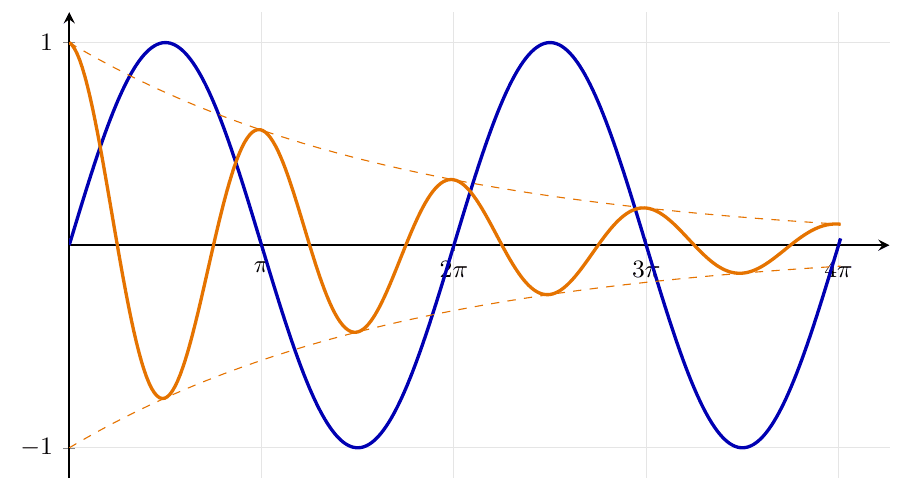
\includegraphics[width=\linewidth]{images/courbes.png}
  \end{columns}
\end{frame}

\begin{frame}{Mathématiques et tableau}
  \begin{equation*}
    \hat{\beta} = (X^\top X)^{-1} X^\top y
  \end{equation*}
  \begin{center}
    \begin{tabular}{lrr}
      \toprule
      Méthode & Temps (s) & Erreur (\%) \\
      \midrule
      A & 1,2 & 3,4 \\
      B & 0,8 & 2,9 \\
      \bottomrule
    \end{tabular}
  \end{center}
\end{frame}

\section{Conclusion}

\begin{frame}{Conclusion}
  \begin{alertblock}{Message principal}
    La dernière diapositive rappelle l'essentiel.
  \end{alertblock}
  \vfill
  \centering
  Merci! Des questions?
\end{frame}

\end{document}
